\chapter{IMPLEMENTAÇÃO}
\quad Neste capítulo é realizada uma discussão sobre a implementação computacional dos algoritmos estudados. O ambiente de desenvolvimento para todos os algoritmos foi o mesmo. O sistema operacional foi o GNU/Linux Ubuntu 15.0.

\quad A implementação foi dividida em etapas. A primeira etapa consiste na captura do áudio, esta foi realizada com a aplicação da biblioteca \textit{alibsound.h}. Esta usa a interface PCM para a modulação do sinal. Nesta fase é necessário checar os parâmetros de hardware através de funções disponibilizadas pela ALSA, documentação disponível em http://www.alsa-project.org/alsa-doc/alsa-lib/pcm.html. Após a captura da onda foi realizado o tratamento da mesma. Foram implementadas funções para aplicação da FFT, DCT, dividir o sinal em frames, aplicar janela de Hamming e por fim extrair caraterísticas do sinal. Nesta fase as principais dificuldades encontradas foram a manipulação de fórmulas matemáticas complexas e o baixo nível de programação. Após a extração das características MFCC é realizada a comparação dos padrões.

\begin{figure}[H]
\centering % para centralizarmos a figura
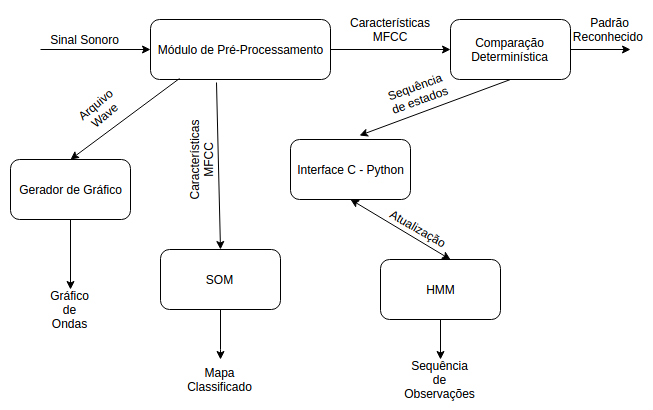
\includegraphics[width=10cm]{img/diaraizatcc.png} % leia abaixo
\caption{Organização dos módulos implementados.}
\label{fig:diatcc}
\end{figure}


\begin{figure}[H]
\centering % para centralizarmos a figura
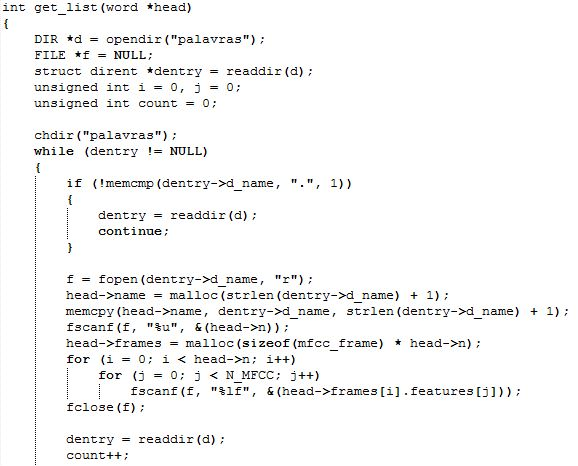
\includegraphics[width=10cm]{img/getlist.jpg} % leia abaixo
\caption{leg1}
\label{fig:getlist}
\end{figure}

\begin{figure}[H]
\centering % para centralizarmos a figura
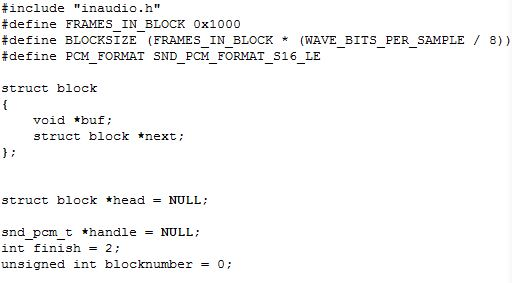
\includegraphics[width=10cm]{img/escinaudio.jpg} % leia abaixo
\caption{leg2.}
\label{fig:inau}
\end{figure}




\section{Comparação de Padrões}
\quad Uma vez havendo extraído as caraterísticas MFCC podemos realizar a comparação entre o padrão de entrada e os
padrões armazenados. Esta comparação pode ser realizada por diferentes algoritmos.




\subsection{Método Determinístico}
\label{sec:det}
\quad O método de comparação de padrão determinístico compara a correlação entre dois vetores de características MFCC, quanto menor o resultado retornado pela função mais parecidos são os padrões. Este algoritmo também foi implementado em linguagem C. Neste método é usado um limiar de correlação para definir se os padrões são iguais. 
\begin{figure}[H]
\centering % para centralizarmos a figura
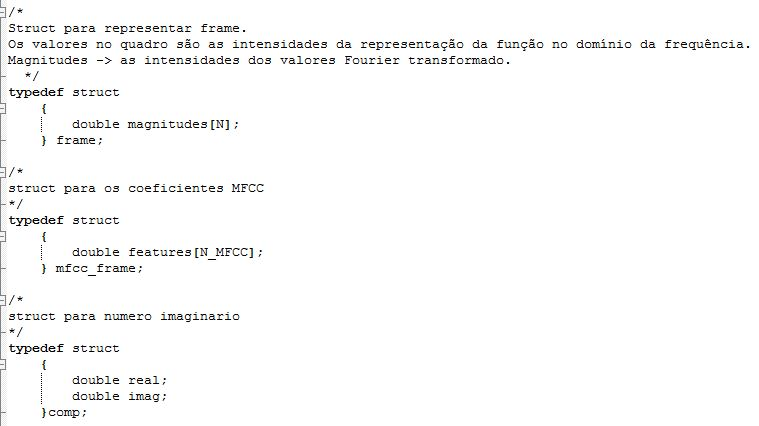
\includegraphics[width=10cm]{img/struct.jpg} % leia abaixo
\caption{leg3.}
\label{fig:str}
\end{figure}



\subsection{SOM}
\label{sec:som}
\quad A implementação do SOM  foi realizada em linguagem de programação C. A principal dificudade encontrada na implementação deste método foi a manipulação do mapa e seus neurônios. O gerenciamento da memória na alocação e liberação de vários ponteiros também se mostrou bastante complexa. O mapa auto-organizável requer  mais memória e tempo na execução do que o método determinístico citado na \ref{sec:det}.


\begin{figure}[H]
\centering % para centralizarmos a figura
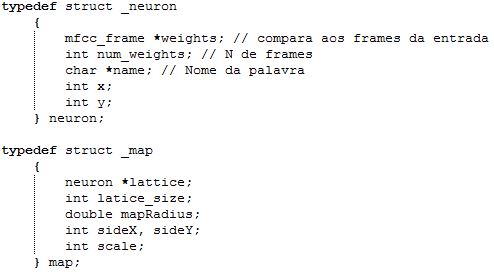
\includegraphics[width=10cm]{img/structneuron.jpg} % leia abaixo
\caption{\textit{Structs} para mapa e neurônio.}
\label{fig:strneu}
\end{figure}



\subsection{HMM}
\label{sec:hmm}
\quad O algoritmo HMM foi implementado em linguagem computacional Python 2.7. Python é uma linguagem de tipagem dinâmica de alto nível, isto facilta na manipulação das estruturas de dados usadas pelo algoritmo.


\begin{figure}[H]
\centering % para centralizarmos a figura
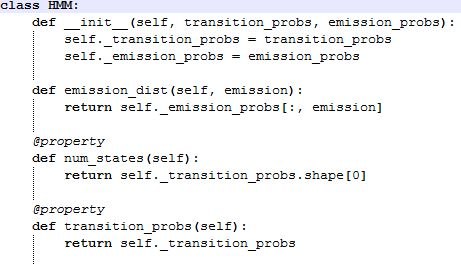
\includegraphics[width=10cm]{img/classhmm.jpg} % leia abaixo
\caption{Classe principal do HMM.}
\label{fig:classhmm}
\end{figure}

